\section{Architecture and Design}\label{sec:architecture-and-design}
The design of the system is approached in three phases: authorization, election,
and delegation. Each phase considers different components of the overall system
architecture and each component is responsible for managing a different set of
responsibilities within the architecture.

% system. The authorization components, delegation components, and election
% components.

% , henceforth collectively referred to as Norman.

% The Embark framework --- a framework designed to build Decentralized
% Applications (DApps) --- is used to provision test networks, build, deploy,
% and test the components. The Embark framework can manage and deploy to
% different chains, e.g., testnet, private net, and livenet. Embark
% automatically detects changes to contracts, builds, and then deploys the
% contracts onto the appropriate Ethereum networks. To build Solidity code into
% EVM code the Embark framework uses solcjs which offers JavaScript bindings for
% the Solidity compiler. For expedited development and testing Embark exposes
% the Ethereum JavaScript testrpc which simulates a fully functioning Ethereum
% client. Interaction with Ethereum contracts is simplified by automatically
% generating promise-based JavaScript functions which expose contract functions.
% JavaScript support is provided by wrapping the web3js library which implements
% the generic Ethereum JSON RPC spec. Embark also supports decentralized storage
% via IPFS, decentralized messaging through Whisper and Orbit, and a curses-like
% dashboard which exposes logs, environment, contract states, available
% services, a console, and the status of the framework generally.

\begin{center}
  \figurepdf{venn-diagram}
  % \includestandalone{\fig{venn-diagram}}
\end{center}

\subsection{Authorization Components}
The authorization components are designed to provide access control: to build
and maintain a set of eligible voters, administrators, and whatever other roles
might be necessary to implement the electoral systems. Ultimately, the
authorization components are responsible for restricting access to sensitive
contract function calls that mutate the state of the contract, e.g., casting
ballots and configuration elections. The design must be flexible enough to
facilitate the varying and evolving needs of different organizations and
communities but consistent enough to support them all through a common
interface. Concepts are borrowed from traditional operating system access
control schemes/models and authorization mechanisms which provide guidance for
system design. The underlying authentication features are handled via the
asymmetric cryptography provided by the underlying blockchain infrastructure.

\subsubsection{Access Control}
Access control schemes exist to authorize access to data and resources; they are
responsible for managing and defining the relationships between permissions,
operations, objects, and subjects. Several access control model schemes were
considered in this phase; among them were: access control lists, discretionary
access control, mandatory access control, and role-based access control.

\paragraph{Discretionary Access Control}
Discretionary Access Control (DAC) is a form of access control where the owner
of some resource/object can dictate the operations and permissions that other
subjects can take on the resource/object. Additionally, the owner of the
resource/object can pass ownership to some other subject. You can see a form of
this in POSIX file systems where ownership over files is granted and transferred
through commands like \codet{chown} and \codet{chmod}.

\paragraph{Access Control Lists}
An Access Control List (ACL) is a collection of \emph{subject}, \emph{resource},
and \emph{permission} relationships which can be understood as a matrix, where
each cell, indexed by \emph{subject} and \emph{resource}, reflects the
\emph{permissions} available for the \emph{subject} to access \emph{resource}.

% \todo{Intersection? Corresponding?}

\paragraph{Role-Based Access Control}
Role-Based Access Control (RBAC) is a form of access control where collections
of permissions are assigned to roles; roles are then assigned to users. In RBAC
roles are hierarchical, thus roles can be inherited from parent roles.

% Word semantic?
\subsubsection{Design}
The fundamental resources exposed by smart contracts are function calls, thus
the security implementation and access control model must revolve around that.
We define an interface, \sol{Authority}, which defines the \sol{canCall}
function. Any contract wishing to implement access control on functions can
leverage a contract that implements the \sol{Authority} interface to authorize
access to those functions.

\begin{figure}[H]
  \centering
  \figurepdf[width=\textwidth]{authorization}
  % 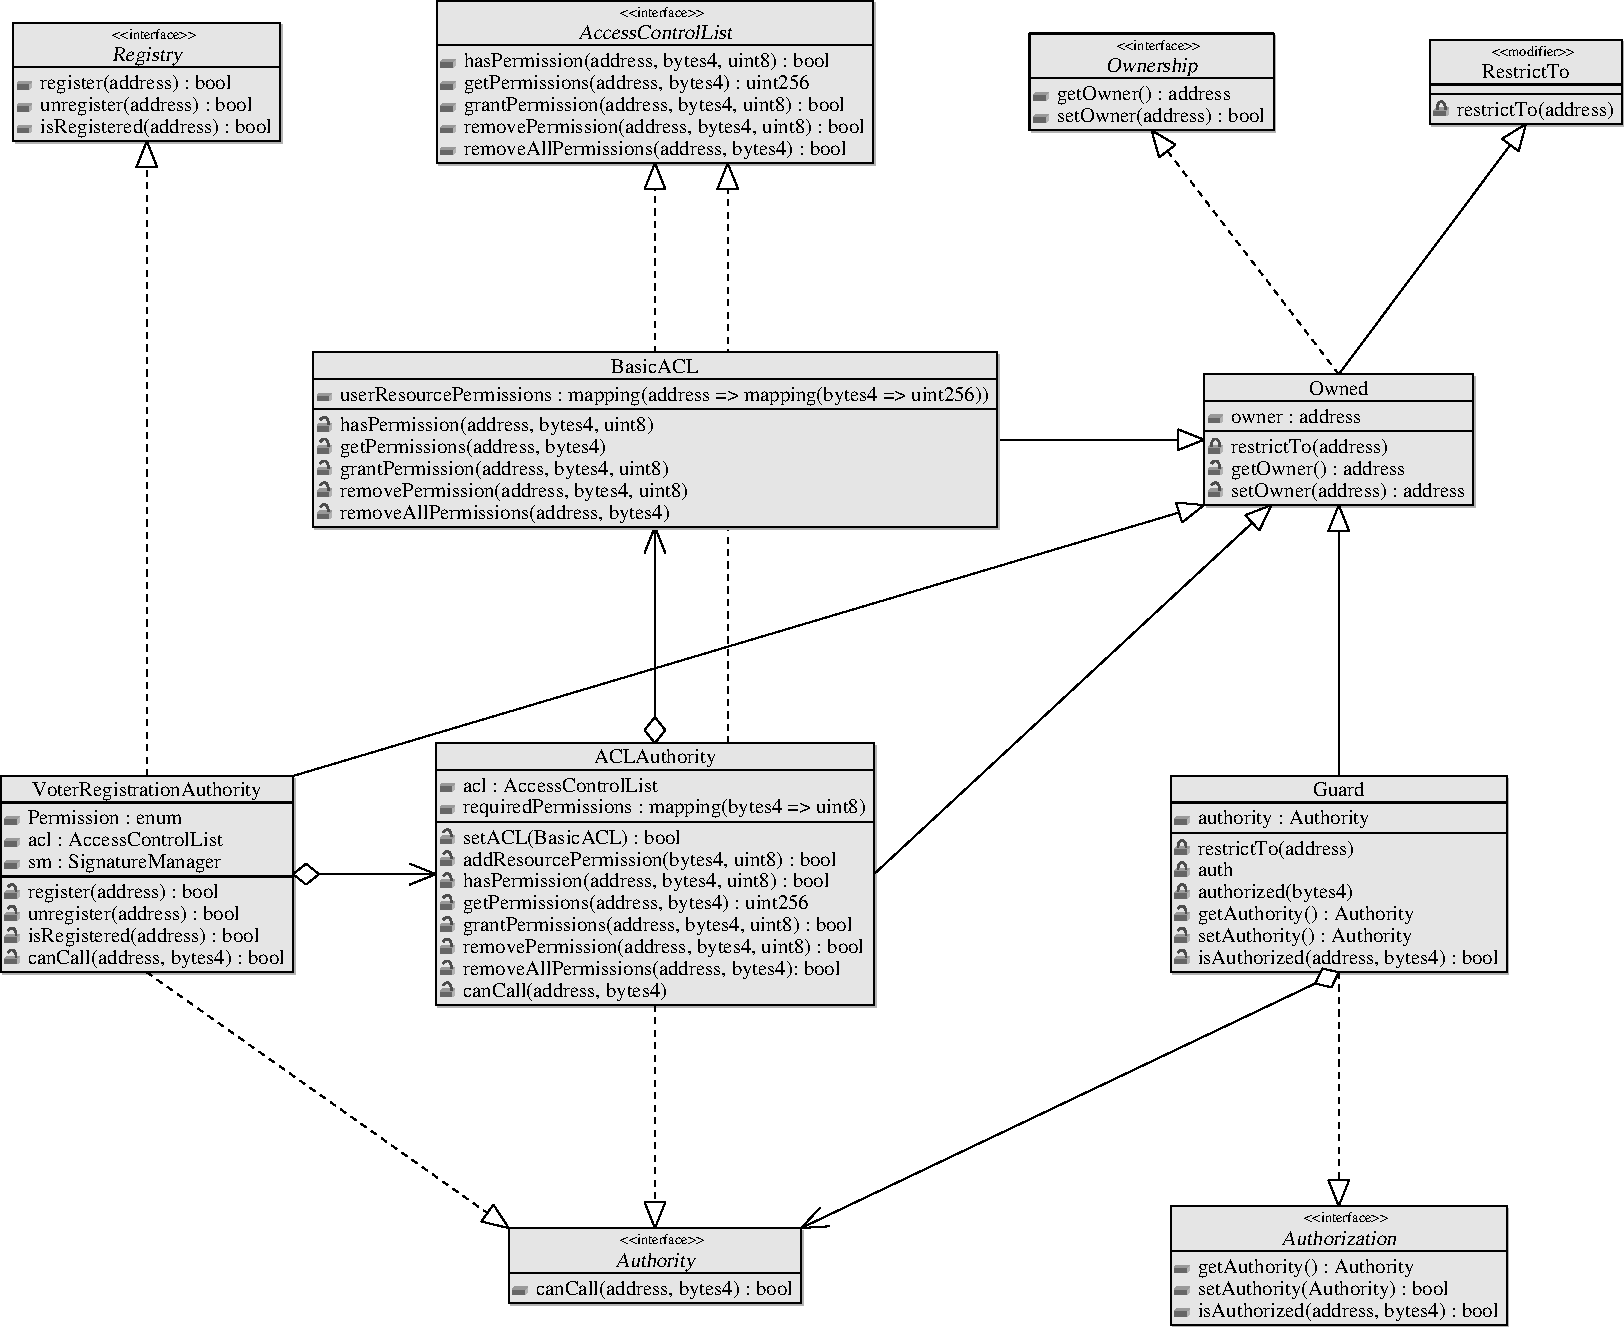
\includegraphics[width=\textwidth]{figures/authorization/figure}
  % \includestandalone[width=\textwidth]{\fig{authorization}}
  \caption{Authorization dependency graph modeling.}\label{fig:authorization}
\end{figure}

We define the \sol{Authorization} interface which offers mechanisms for
interacting with an \sol{Authority}. This interface defines \sol{getAuthority},
\sol{setAuthority}, and most importantly, \sol{isAuthorized}. A contract that
realizes the \sol{Authorization} interface is expected to aggregate an
\sol{Authority} but does not necessarily need one externally; for example, a
contract that provides \sol{Authorization} may also be its own \sol{Authority}.
Likewise, an \sol{Authority} can provide its own \sol{Authorization}. The
\sol{Authority} and \sol{Authorization} interfaces together form our access
control primitives.

The \sol{Guard} contract realizes the \sol{Authorization} interface and provides
the modifier functions \sol{auth} and \sol{authorized}. These can be applied to
other functions to easily restrict function-call access to accounts that the
\sol{Authority} has approved, e.g.,

\begin{solidity}[Guard Usage Example]
function sensitive () public auth returns (bool _success) {
  // The `auth` modifier prevents this function from being
  // called until the Authority has confirmed that the
  // the message sender has the proper privileges.
  return true;
}
\end{solidity}

This implementation conforms to a number of design principles: separation of
concerns, dependency inversion principle, open/closed principle, interface
segregation, substitution principle, and single responsibility principle.
Ultimately it provides the flexibility and resiliency necessary to build out a
wide variety of electoral systems.

\paragraph{Ownership}
Access control often starts before our \sol{Authority} and \sol{Authorization}
realizations. Most contracts offer a primitive form of access control through
\sol{Ownership}. All contracts and most contract functions are open and public
by design; thus, it is important to lock down sensitive contract functions from
deployment. A common pattern is to store the \solt{address} of the creator of a
contract as an owner in the contract state and to use that address to restrict
access to sensitive public-facing functions. More complicated ownership
mechanisms can be built using this pattern by leveraging contracts which
delegate ownership to another contract which can then define more complex access
control and management mechanisms. To facilitate in this and many other useful
patterns we introduce a simple \sol{Ownership} interface. The \sol{Ownership}
interface defines functions \sol{getOwner} and \sol{setOwner} which get and set
the account address of a contract's owners respectively.

To facilitate in restricting access of functions to a single account we also
define a contract \sol{RestrictTo} that provides a modifier function
\sol{restrictTo}. The \sol{restrictTo} modifier can be applied to any other
function and takes an account address argument; if the address of the account
calling a \sol{restrictTo} modified function does not match the argument
provided to \sol{restrictTo} (often the owner), then the function will
immediately exit and revert any changes to the contract. Finally, we realize and
extend these two contracts to form the concrete \sol{Owned} contract. This
pattern is so ubiquitous that most, if not all, concrete contracts in our
governance ecosystem will extend this contract.

\paragraph{Authority}
We need to provide access control beyond interfaces, standards, and single
account address restrictions. Our access control implementation leans towards
access control lists as a primitive that can be extended to provide other access
control mechanisms such as role-based access control. Alternatively, a contract
can realize the \sol{Authority} interface itself if ACLs are not a useful
abstraction.

\subparagraph{Access Control List}
We first define an ACL interface, \sol{AccessControlList}, which defines basic
ACL functionality: \sol{hasPermission}, \sol{getPermissions},
\sol{grantPermission}, \sol{removePermission}, and \sol{removeAllPermissions}.
The design supports assigning up to 256 unique permissions per contract
signature.

\subparagraph{Basic ACL}
Next we realize a concrete implementation of the \sol{AccessControlList}
interface named \sol{BasicACL}. \sol{BasicACL} is primarily a
database contract which creates a mapping from account address to a mapping of
functions (the first 4 bytes of their signature) to an unsigned 256-bit integer
that represents the permissions. This implementation is similar to what can be
found in POSIX compliant operating systems. In Java one might represent this
access control model as \codet{HashMap<Account, HashMap<Function,Permission>>}.

Naturally \sol{BasicACL} provides implementations for the functions defined by
\sol{AccessControlList}: \sol{hasPermission}, \sol{getPermissions},
\sol{grantPermission}, \sol{removePermission}, and \sol{removeAllPermissions}.
These work using bitwise NOT, OR, and AND operations to modify the 256-bit
unsigned integer representing permissions for a particular (account, function)
pair.

\subparagraph{ACL Authority}
We can easily build an \sol{ACLAuthority} out of our \sol{BasicACL} using the
adapter pattern and aggregation. We simply aggregate an instance of a
\sol{BasicACL} and realize the \sol{Authority} and \sol{AccessControlList}
interfaces. Finally, we lean on the \sol{hasPermission} function to implement
our \sol{canCall} function which presumably forwards our request to a
\sol{BasicACL} instance and returns the result. This structure also allows us to
implement a composite pattern and aggregate many trusted authorities into one.

\subparagraph{Voter Registration Authority}
Our final step is to use a facade to hide the more complex implementation
details from outside contracts. We introduce a \sol{VoterRegistrationAuthority}
which realizes the \sol{Registry} and \sol{Authority} interfaces.
The \sol{Registry} interface provides some nice abstractions:
\sol{register}, \sol{unregister}, and \sol{isRegistered}. We
presume the contract aggregates some number of \sol{AccessControlList}s as
a foundation for its \sol{Registry} function implementations, but does not
need to necessarily. Finally, the \sol{canCall} function leans on the
\sol{Registry} functions, specifically \sol{isRegistered} to grant
access to functions.

The end result is a clean, public, and composable voter registration authority.


\subsection{Election Components}
The election components are responsible for constructing and operating election
processes. These responsibilities include maintaining the integrity and security
of the election, handling votes, tallying ballots, and determining election
winners.

The phases typically involved in conducting an Internet-based election,
described in Section~\ref{sec:internet-voting}, are: Setup, Distribution,
Voting, Casting, Tallying, and Auditing. Responsibilities pertaining to voter
registration, which are typically handled in the Setup phase, are expected to be
managed by Authorization components. The Distribution phase, which mostly
pertains to processes such as mailing election materials to voters, is
considered outside the scope of this research and therefore ignored. The
Auditing phase, where election integrity and results are scrutinized, is assumed
to be handled and provided by the underlying features made available by
Ethereum.

% Ideally the ballots would be recorded separately from the tallying method. If
% they were we could apply different tallying methods to the same set of ballots
% and produce different results. Unfortunately it's extremely costly to store
% ballots as part of the contract state.

% We opt for first-past-the-post and range vote for single-winner elections, the
% former for its simplicity and ubiquity, the latter for its effectiveness. This
% provides an implementation of a plurality voting system and majority voting
% system.

\subsubsection{Design}
Each electoral system implementation is unique, due mostly to the unique
requirements necessitated by their underlying tallying algorithms and ballot
structures.

There are important electoral criteria worth considering when analyzing the
implementation feasibility of these electoral systems, namely, the ballot
counting criteria: summability, polynomial time, and resolvable. These electoral
criteria are significant because they impact the gas costs associated with
operating the electoral system. Table~\ref{tab:criteria-compliance} is a useful
resource when considering these electoral criteria. Both the first-past-the-post
and range vote electoral systems are a 1\textsuperscript{st}-order summable;
i.e., ballots can be tallied using a linear amount of space with respect to the
number of choices available without losing information required to complete the
tallying processes. Both also have polytime ballot counting implementations that
are linear in the number of candidates and voters. STV is not listed in the
table; however, its single-winner equivalent (IRV) is; which implies that STV
has, at best, a tallying complexity of $O(n^2)$ and a summability complexity
of $O(n!)$ with respect to the number candidates.

Gas costs must be considered when implementing, deploying, and running contract
functions on the Ethereum Virtual Machine (EVM). If gas costs are too high then
it may become infeasible for an external account to afford to execute a contract
function, e.g., the network fees become too high to vote. Another concern to
consider is that the cost to execute a contract function may become too high to
ever complete in a single block, therefore never actually complete. The most
expensive operations, by no small margin, are operations involving storage.
Therefore it is important to minimize storage usage.

% Fortunately these EVM limitations map well
% to many voting method criteria. We can lean on these criteria and the field of
% computational social choice theory broadly to restrict the set of voting systems
% to just the ones that can be feasibly implemented on the Ethereum blockchain.

\paragraph{Finite State Machine}
Several of the voting system designs use a phased approach with timed
transitions between election states: Configuration, Frozen, Vote, and Tally.
These phases can be modeled as a finite state machine where calls to various
functions trigger transitions to different stages. A modifier function can be
used to restrict access of functions to only be callable during their
appropriate state. Most of the transitions from state to state can be designed
as timed transitions which occur lazily, i.e., the check to confirm that it is
time to transition from one state to another occurs when a function is called.
The rationale for this approach is due to the fact that Ethereum offers no
mechanism to trigger code execution \emph{from within the blockchain itself};
therefore all function calls, even if called from another function or even a
function in a different contract, must ultimately have originated from a
transaction created by an externally owned account. The product of this timed
transition implementation implies that the state restriction modifier needs to
occur after the lazily evaluated timed transition modifier; i.e., first update
the current state if it should be, then validate if the function should
executed. On the other hand, if transitions are manually updated during a
function's execution then the opposite behavior should occur; i.e., first
validate if the function should be run, then update the state as required.

\subparagraph{Configuration}
The Configuration phase, as implied by the name, exists to provide election
administrators an opportunity to configure the election contract: choices,
election start/end time, etc. After the configuration is complete the
administrators can freeze the contract, preventing it from being modified
further.

\subparagraph{Frozen}
Transitioning to the Frozen phase could simply set a boolean \sol{frozen} to
true and update the phase to Frozen. The boolean \sol{frozen} should be checked
at the start of every administrative function's execution and should cause the
immediate cease of code execution if the value is true. This serves to prevent
potentially malicious election administrators from modifying an election
contract after the voting process has started; it also serves to notify external
contracts and users that the election is configured and is ready or waiting to
move into the Vote phase.

\subparagraph{Vote}
The Vote phase is the phase during which various kinds of voting can occur for a
particular election contest. A \sol{vote} function should be defined. For
flexibility, a \sol{vote (uint8[], uint8[])} function signature is considered
which is capable of being leveraged by most kinds of electoral systems and
ballot structures. For example, as a sparse vector, where both arrays are of
equal length; values in the first array act as a choice index and values from
the second array act as a choice value. This could be used to marginally reduce
the size of transactions for many kinds electoral systems.

\subparagraph{Tally}
The Tally phase is the final phase of the election process that takes place
after the end of the Voting phase. The exact tallying process will depend on the
electoral system itself.


\paragraph{First-Past-the-Post}
The process for a first-past-the-post election is as follows:

\begin{enumerate}
  \item Configuration
  \begin{enumerate}
    \item Election administrators add each contest choice: \\
      \sol{addChoice(bytes32 _choice)}.
    \item Election administrators set the voting start time: \\
      \sol{setVoteStartTime(uint _voteStartTime)}.
    \item Election administrators set the voting end time: \\
      \sol{setVoteEndTime(uint _voteStartTime)}.
    \item Election administrators freeze the electoral contract, preventing
      further contract configuration mutations: \sol{freeze()}.
  \end{enumerate}

  \item Frozen
  \begin{enumerate}
    \item All functions are disabled until start time is met.
  \end{enumerate}

  \item Vote
  \begin{enumerate}
    \item Authorized voters cast votes by calling the \sol{vote(uint8 _choice)}
      function, where the value provided is the choice the voter supports.
      Votes are immediately summed into the struct of the appropriate choice.
      This is feasible because the first-past-the-post electoral system is
      summable in linear time and with linear space consumption.
  \end{enumerate}

  \item Tally
  \begin{enumerate}
    \item When the voting end time is reached the election moves into the
      Tally phase. At this point only the tally function can be called.
      The tally function, in this case, will check the number of votes for
      each candidate and set the winner to the choice that has received
      the most support. The election administrator is expected to run this
      contract function but any account can execute this function without
      any consequence to the result of the contract.
  \end{enumerate}
\end{enumerate}

\paragraph{Range Voting}
The process for a range vote is very similar to the process for
first-past-the-post. It is as follows:

\begin{enumerate}
  \item Configuration
  \begin{enumerate}
    \item Election administrators add each contest choice: \\
      \sol{addChoice(bytes32 _choice)}.
    \item Election administrators set the voting start time: \\
      \sol{setVoteStartTime(uint _voteStartTime)}.
    \item Election administrators set the voting end time: \\
      \sol{setVoteEndTime(uint _voteStartTime)}.
    \item Election administrators set the max score (<=100) a choice can
      receive: \\
      \sol{setMaxScore(uint8 _maxScore)}.
    \item Election administrators freeze the electoral contract, preventing
      further contract configuration mutations: \sol{freeze()}.
  \end{enumerate}

  \item Frozen
  \begin{enumerate}
    \item All functions are disabled until start time is met.
  \end{enumerate}

  \item Vote
  \begin{enumerate}
    \item Authorized voters cast votes by calling the \sol{vote(uint8[] _choices, uint8[] _scores)}
      function. The parameters act as a sparse vector where the value
      provided in \sol{_choice} indicates the choice being scored
      and the corresponding value provided in \sol{_scores}
      indicates the score of the choice. Scores are immediately summed
      into the struct of of the appropriate choice and a
      \sol{voteCount} member is incremented. This is feasible
      because the range vote electoral system is summable in linear time
      and with linear space consumption.
  \end{enumerate}

  \item Tally
  \begin{enumerate}
    \item When the voting end time is reached the election moves into the
      Tally phase. At this point only the tally function can be called.
      The tally function for this electoral system will, for each choice,
      multiply the summed score by $10^p$ where $p$ is
      \sol{precision} then divide the result by
      \sol{voteCount} to find an average score for the choice. The
      winner is set to the choice with the highest average score. The
      score is multiplied by $10^p$ because the EVM does not have floating
      point functionality and a greater precision makes ties less likely.
      The election administrator is expected to run this contract function
      but any account can execute this function without any consequence to
      the result of the contract.
  \end{enumerate}
\end{enumerate}



\subsection{Delegation Components}
The delegation components offer mechanisms for the electorate to vest votes to
delegates who may vote on their behalf. A delegation hierarchy lends itself to a
graph representation.\cite{delegative-democracy} Specifically a directed
acyclic graph (DAG) forest-like structure where pendant and isolated vertices
represent voters and all other vertices represent delegates. A sink vertex
represents a delegate who has not delegated their vote further. Directed edges
represent delegations. The total weight of a voter, their voting power, can be
measured by recursively calculating the total number of incoming edges for each
vertex. We represent edges in the graph as follows:

% \begin{displayquote}
%   In a large and complex organization, the generalist role --- merely knowing
%   who knows best about something --- is often as important a function as the
%   specialist role of being able to make good decisions in any particular area.
%   In traditional large democratic structures, where elected officials in key
%   positions manage a hierarchical bureaucracy of some kind, most of those
%   elected positions are effectively generalist positions by practical necessity.
%   Ordinary voters do not have the interest level or patience required for
%   electing appropriate people to a large number of specialist positions, and
%   most would not have the knowledge or connections required to make good
%   decisions about those positions anyway. Therefore, specialists can usually
%   only participate in a large organization by being appointed or hired into a
%   position in the un-elected bureaucracy, and for this reason people are always
%   effectively subservient to the generalists who choose them. For this reason
%   the entire field of ``politics'' has effectively become a profession of
%   generalists, which very little technical knowledge in any particular field is
%   required or expected (except perhaps law), but in which the most important
%   characteristic of a candidate is the ability to look good, speak well, and
%   make the right connections. But it seems unfortunate and problematic that all
%   specialists are effectively excluded from direct participation in the
%   democratic process except in role that are strictly subservient to the
%   generalists: at the very least this structural pathology certainly contributes
%   to the frequently observed tendency of politicians to ``legislate'' highly
%   technical issues without adequate consultation with the experts in the
%   appropriate technical field --- or with a selection of ``experts'' that is
%   highly skewed for political reasons --- often with disastrous results.
%   Delegative democracy with open specialized forums and re-delegation provides
%   an alternative structure that enables both generalists and specialists to
%   participate directly in the democratic process as first-class policy-makers.
%   Widely recognized and trusted generalized are given the legitimate ability to
%   affect the balance of power in specialized forums by directing delegated votes
%   to chosen specialists, while the specialists participating directly in those
%   forums also retain the ability to build their own independent power bases and
%   thus not be completely at the mercy of generalists. At the same time, since
%   generalists and specialists alike are direct participants in the democratic
%   process, they have the same fundamental rights and responsibilities and are
%   all held accountable to all of their constitutes (i.e., those who delegate
%   votes to them) in the same way.
% \end{displayquote}

\begin{solidity}[Delegation Structure]
struct Voter {
  uint40 weight; // 5 bytes
  address delegate; // 32 bytes
}
\end{solidity}

Each time a delegation occurs a depth first traversal should be performed to
ensure that no cycles are created by the delegation; doing so maintains the
acyclic invariant required of the graph to support voter delegation. A simple
graph coloring algorithm is considered, beginning with white vertices and
coloring vertices black as they are traversed; traversal starts from the vertex
representing the voter who is delegating their vote and ends at some sink
vertex. If no cycle is detected the algorithm should check to see if the voter
has already delegated their vote; if so, it should traverse down their current
delegation path, decreasing the weight of each vertex visited by the weight
of the voter or delegate delegating their vote. Finally, the algorithm should
record the new delegate address and perform a final traversal, following the
same path originally traversed while performing cycle detection, increasing the
weight of each vertex visited along the way by the weight of the voter or
delegate delegating their vote. More briefly:
\begin{enumerate}
  \item Confirm that there are no cycles within the new delegation chain.
  \item Decrease the weight of the delegates in the old delegation chain.
  \item Increase the weights of the delegates in the new delegation chain.
\end{enumerate}
A complete implementation of this algorithm is as follows:\footnotemark{}

\footnotetext{
  Here we assume that every voter has their voting weight initialized to 1. This
  algorithm might be improved by combining the cycle detection and weight
  accumulation steps while leveraging the \sol{revert()} function to revert the
  state of the contract if a cycle is detected. We opt not to do that for now
  because return values are not currently available with the \sol{revert()}
  functionality.
}

\begin{solidity}[Vote Delegation]
mapping (address => Voter) voters;

function delegateVote (address delegate) public auth returns (bool _success) {
  // The `auth` modifier prevents this function from being
  // called until the Authority has confirmed that the
  // the message sender has the proper privileges.
  Voter cursor;
  uint40 weight = voters[msg.sender].weight;

  mapping (address => bool) visited;
  visited[msg.sender] = true;
  visited[delegate] = true;

  // Cycle Detection
  cursor = voters[delegate];
  while (cursor.delegate) {
    address newDelegate = cursor.delegate;
    if (visited[newDelegate]) return false;
    cursor = voters[newDelegate];
    visited[newDelegate] = true;
  }

  // Decrement weights of old delegate chain.
  cursor = voters[msg.sender];
  while (cursor.delegate) {
    address newDelegate = cursor.delegate;
    cursor = voters[newDelegate];
    cursor.weight -= weight;
  }

  // Increment weights of new delegate chain.
  cursor = voters[msg.sender];
  cursor.delegate = delegate;
  while (cursor.delegate) {
    address newDelegate = cursor.delegate;
    cursor = voters[newDelegate];
    cursor.weight += weight;
  }

  return true;
}
\end{solidity}



